\documentclass[10pt,twocolumn,letterpaper]{article}

\usepackage{cvpr}
\usepackage{times}
\usepackage{epsfig}
\usepackage{graphicx}
\usepackage{amsmath}
\usepackage{amssymb}

% Include other packages here, before hyperref.
\graphicspath{{../figures/}}

% If you comment hyperref and then uncomment it, you should delete
% egpaper.aux before re-running latex.  (Or just hit 'q' on the first latex
% run, let it finish, and you should be clear).
\usepackage[pagebackref=true,breaklinks=true,letterpaper=true,colorlinks,bookmarks=false]{hyperref}

\cvprfinalcopy % *** Uncomment this line for the final submission

\def\cvprPaperID{****} % *** Enter the CVPR Paper ID here
\def\httilde{\mbox{\tt\raisebox{-.5ex}{\symbol{126}}}}

% Pages are numbered in submission mode, and unnumbered in camera-ready
\ifcvprfinal\pagestyle{empty}\fi
\begin{document}

%%%%%%%%% TITLE
\title{Quantifying redundancy in natural image patches}

\author{Niru Maheswaranathan\\
Stanford University\\
\textit{nirum@stanford.edu}
% For a paper whose authors are all at the same institution,
% omit the following lines up until the closing ``}''.
% Additional authors and addresses can be added with ``\and'',
% just like the second author.
% To save space, use either the email address or home page, not both
%Second Author\\
%Institution2\\
%First line of institution2 address\\
%{\tt\small secondauthor@i2.org}
}

\maketitle
\thispagestyle{empty}

%%%%%%%%% ABSTRACT
\begin{abstract}
The space of natural images is both high-dimensional and has striking non-Gaussian, higher-order statistical structure. It has been argued on information theoretic grounds that much of early visual processing consists of removing statistical regularities in visual input, in what is known as the redundancy reduction hypothesis. A key part of understanding the redundancy of natural scenes is understanding the entropy of image patches. Entropy allows us to quantify the information content of image patches, and bounds optimal compression schemes. This project aims to characterize the redundancy of natural images by quantifying the entropy of both the raw ensemble of images as well as other generative models of natural images.
\end{abstract}

%%%%%%%%% BODY TEXT
%\noindent\large\textbf{Future Distribution Permission}\\
%\indent The author(s) of this report give permission for this document to be distributed to Stanford-affiliated students taking future courses.

%\section{Problem statement}
%\section{Outline}
%\begin{itemize}
    %\item \textbf{Motivation:} why do we care about the statistics of natural images?
    %\item What insight does this give us for computer vision?
    %\item Reduced descriptions of natural images: can we compress images as a pre-processing step for CV algorithms?
    %\item Inspiration side Note: let's see what the brain does
    %\item why entropy? why info theory?
    %\item \textbf{Background:}
    %\item Entropy of image patches. sparsity of pixel distributions
    %\item Redundancy reduction, PCA, sparse coding/ICA (figure 1)
    %\item sparsity of feature distributions
    %\item \textbf{Results:}
    %\item Entropy estimation via kernel density estimation
    %\item Entropy estimation via nearest neighbor techniques
    %\item Comparison of the methods for Gaussian models, and 1D non-Gaussian distributions
    %\item Entropy estimation of raw (unprocessed) image patches
    %\item Entropy estimation of reduced descriptions of images (PCA, ICA, random bases?)
    %\item \textbf{Evaluation:}
    %\item make it clear: since the entropy is an unknown, high-D quantity, we have no ground truth. We can only trust that since the method works for arbitrary low-D distributions, and high-D gaussians, that it works for high-D arbitrary distributions.
    %\item Comparison of results with other results from the literature.
%\end{itemize}

\section{Introduction}
It has long been argued \cite{barlow} that the human visual system has evolved to efficiently process the statistical structure of natural images. This suggests that computer vision systems can also be tuned to the structure of natural images. A useful metric for quantifying the redundancy in the distribution of image patches is the entropy of the distribution. Entropy can be thought of as a measure of the information content of a distribution, therefore, the entropy of the distribution of natural scenes bounds the amount of information available to vision systems (either man-made or in nature). Entropy also provides a lower bound on the number of bits needed for compression, thus knowledge of the entropy of natural images gives us an absolute threshold with which to compare compression schemes.

\subsection{Motivation and significance for computer vision}
Broadly stated, computer vision systems attempt to extract meaning from natural images.
Knowledge of the statistical structure of images is useful from this perspective for a number of reasons.
First, it lets us place priors on Bayesian inference models. Given noisy data (such as a recorded visual scene), we would like to infer the causes of that data, and therefore need a good model for the prior over the statistics of natural images.
Secondly, redundancy plays a key role in the study of compression schemes. From Shannon we know that the entropy of a distribution bounds the optimal compression we can achieve given any compression scheme. This lets us put compression algorithms for images on an absolute scale.
Finally, the statistics of images is key to understanding useful pre-processing steps for computer vision systems, as well as for finding useful features or basis sets for describing key parts of images in a compact representation (then useful for training machine learning algorithms).
I would like a more rigorous understanding of why certain features or representations are better than others, and at a low-level, this is related to the statistics of image patches.

An important unknown that is critical to these goals is understanding the nature and strength of redundancy in natural images, which is the focus of this work.

%Quantitative comparisons have shown that these response properties are not all equally effective in removing statistical dependencies \cite{nicv1}.
%It is unclear whether neural response proper- ties in cortex can still be interpreted convincingly in terms of redundancy reduction (Eichhorn, Sinz, \& Bethge, 2009).
%entropy is the theoret- ical limit of compression – the lower bound on any compression scheme.

\subsection{Background}
A few previous studies \cite{petrov,chandlerfield} have developed methods for estimating the entropy of image patches. Chandler and Field use an approximation that relies on nearest-neighbor (NN) distances. For $8\times8$ patches, they need around $2^{16}$ samples to correctly estimate the entropy. It has been shown \cite{entropyest} that the average log NN distance can be used to estimate the entropy without estimating the probability distribution $p(x)$. Another approach involves fitting maximum entropy models to natural images. These models are guaranteed to have the largest entropy given certain statistics observed from data. This was the approach taken by \cite{maxen}, who fit an approximate maximum entropy model and used it to estimate the entropy of image patches.
Here, I focus on using nearest-neighbor methods for estimating entropy.

In addition to entropy estimation, an active area of research is in methods of reducing the redundancy of natural images.
One way of acheiving this is to run algorithms on image ensembles that look for linear projections that remove correlations or higher order dependancies in images \cite{nis}.
Work from others \cite{bethge,nicv1} assesses the effectiveness of various basis functions in eliminating redundancy in image descriptions.
Redundancy reduction provides a way of encoding images using fewer bits, and is also thought to be one of the principles of sensory coding in the brain \cite{barlow}.

\begin{figure*}[h]
\begin{center}
%\fbox{\rule{0pt}{2in} \rule{.9\linewidth}{0pt}}
   \includegraphics[width=0.8\textwidth]{example_patches.png}
   \caption{Sample natural image patches (top) and probability distribution over single pixel values (bottom)}
    \label{fig:ex}
\end{center}
\end{figure*}

\section{Methods}
I treat image patches as a point in an $N$ dimensional space, where $N$ is the number of pixels in each patch.
A broad goal is to understand the statistics of the set of all $N$ dimensional patches.
Here, we focus on three descriptions of these statistics: pairwise pixel statistics, the entropy of patches, and the entropy of patches projected onto reduced descriptions of images.
By reduced description, I mean images projected on to a low-dimensional feature set or basis.

\subsection{Dataset}
The dataset used for obtaining samples of natural images is the van Hateren natural image database \cite{vanhateren}.
This is a widely used dataset, consisting of 4212 images, each containing 1536 by 1024 pixels. The images consist of outdoor scenes, wooded areas, landscapes and buildings. The specifics of the larger scene do not matter here, as we are interested in the statistics of small image patches. Figure \ref{fig:ex} shows a few $64\times 64$ image patches sampled from the dataset, along with the distribution of single pixel intensities sampled from 100 such patches.

\subsection{Reduced descriptions of images}
In addition to studying redundancy in raw distributions of image patches, we are also interested in "reduced descriptions" of images, that is, the distribution of images projected onto some feature basis. Here, we restrict our attention to the two most common bases used in describing natural images: principal and independent components analysis (PCA and ICA, respectively). In prinicpal components analysis, we project image patches onto the top $k$ eigenvectors of the covariance matrix, equivalent to the description used in the Eigenfaces algorithm. Interestingly, since image patches are translation invariant, the eigenvectors are Fourier modes, so PCA is effectively performing a Fourier transorm on the image patch. This is related to the observation that the amplitude spectra of natural images is inversely proportional to frequency (has $1/f$ structure). Learned PCA basis vectors are shown in Figure \ref{fig:bases}(a).

{\small
\centering
\begin{figure}
   \includegraphics[width=1.0\linewidth]{bases.jpg}
   \caption{Learned basis vectors using algorithms for redundancy reduction}
   \label{fig:bases}
\end{figure}
}
\noindent In ICA, the objective is to remove all correlations in the data (second order and beyond) \cite{ica}. When one runs ICA on natural image patches, the resulting features are oriented and bandpass, and strongly resemble receptive fields recorded from visual area V1 in the brain \cite{nis}. Learned ICA basis vectors from $32\times 32$ image patches are shown above in Figure \ref{fig:bases}(b).

\subsection{Entropy Estimation}
I use two methods to estimate the entropy of image patches, kernel density estimation (KDE) and a nearest-neighbor (NN) method. Kernel density estimation (KDE) involves estimating the density $p(x)$ as follows:
\begin{eqnarray}
    p(x) = \frac{1}{n}\sum_{i=1}^n K(x-x_i)
\end{eqnarray}
Where $K(\cdot)$ is the kernel (a symmmetric function that integrates to one). Here, we use Gaussian kernels, that is, $K(x)$ is chosen to be the normal distribution. This method is only efficient for low-dimensional distributions, as many samples are needed to correctly estimate the probability density function.

The difficulty in estimating the entropy of image patches arises due to the curse of dimensionality: for patches of size $n\times n$, we must estimate a probability distribution with dimension $n^2$, which quickly becomes infeasible as $n$ grows. Despite these limitations, people have recently made estimates of the entropy using approximate methods.

Here, we use an approximation that relies on nearest-neighbor (NN) distances. It has been shown \cite{entropyest} that the average log NN distance can be used to estimate the entropy without estimating the probability distribution $p(x)$. More specifically, the entropy estimate $H_n$ given $n$ samples from the distribution $p(x)$ can be written as follows:
\begin{eqnarray}
    H_n = \frac{1}{n}\sum_{i=1}^n \log(n\rho_{n,i}) + \log(2) + C_E
\end{eqnarray}
Where $C_E$ is the Euler constant, $C_E = -\int_0^\infty e^{-t} \log(t) dt$, and $\rho_{n,i}$ is the Euclidean distance of the nearest-neighbor of the sample $X_i$:
$$ \rho_{n,i} = \min_{j\neq i} ||X_i - X_j||$$
\noindent Intuitively, we can think of this as a rough measure of the spread in our distribution, which is in turn related to the entropy.
The advantage of this estimate is that it scales better with the dimension $d$ of the data than a kernel density estimate.

\subsection{Computational complexity}
In order to estimate entropy using nearest neighbor techniques, we still need to compute the Euclidean distance between all pairs of samples, which takes $\mathcal{O}(N^2)$ operations. To estimate the entropy of high dimensional distributions, we need many samples, therefore the runtime quickly grows unwieldy as we increase the dimension of the distribution. To improve runtime, I wrote a C++ mex function to compute Euclidean distances between samples. Using this function, entropy estimation took over hours for $10^5$ samples on the Corn cluster (see Figure \ref{fig:entropy}).

%\section{Evaluation}
%The ultimate goal of this project is to obtain plots of the entropy (in bits per pixel) of image patches for different patch sizes.

%To validate the methods, a comparison of how the various metrics perform when estimating image patches drawn from known distribuitons with fixed statistical structure (white/colored noise) will be used as a baseline for comparison, since the entropy of these distributions is known analytically.

%Once the methods have been validated, entropy estimates of the different measures on natural image patches will be compared. Different curves will be shown for measures of the entropy made using different methods. Another criterion for evaluation is comparing the consistency of different entropy estimates for increasing sample sizes.

%Finally, these results will be compared with recent entropy estimates from the literature [refs].

%\section{Preliminary Results}
%As described above, I have used a one-dimensional distributions as a baseline for comparing entropy estimation methods. Figure 2 shows the two methods' (kernel density and nearest-neighbor) estimates of the entropy of samples from a univariate normal distribution, along with the (analytically known) true entropy. We see that the estimates converge at similar rates and yield accurate estimates with roughly $10^3$ samples. Estimating with $10^4$ samples already takes a few seconds on my laptop, as computing the nearest-neighbors takes $N^2$ operations.

%We can also estimate the entropy on the distribution of pixel intensities drawn from natural images, shown in Figure 3. Here, there is no analytical estimate, but we see that both the kernel density estimate and the nearest-neighbor estimate converge to around 6.5 bits per pixel.

%I have implemented the nearest neighbor algorithm to estimate the entropy of a sampled distribution. In Section (???), I compare this method to a simple kernel density estimate of the entropy of a 1D Gaussian and show how they converge for increasing sample sizes. In Section (???), I apply the same methods to estimate the entropy of samples of single pixel intensities (another 1D distribution). Finally, I have also run the algorithm on N-dimensional distributions, image patches sampled from both whiten oise and natural images. These are discussed in Section ???

%\subsection{1D Distributions}
%To test the implementation of the algorithm, I first tested it on one-dimensional distributions, where the estimate could be compared to estimates via other techniques. Specifically, I tested

%Algorithms for entropy estimation (KDE and NN)

%Estimation of a 1D gaussian (compare to theoretical result)

%Estimation of other 1D distributions with known entropy

%Estimation of distribution of pixel intensities

%Estimation of N-dim gaussian

%\section{Current Challenges and Future Work}
%The biggest challenge I am currently facing involve computational complexity. The previous work needed to go out to $10^8$ or so samples to get accurate estimates of the entropy for large (8x8) pixel patches. To do this, I think I would have to offload the computation to corn or another cluster. There is also a trade-off between CPU and memory resources, as the distance computation can be done faster in parallel in matlab although it requires a lot of memory for large sample sizes.



%While estimating the entropy of the raw distribution of images is a nice first step, I am also very interested in comparing estimates of the reduced descriptions of natural images. By reduced descriptions, I mean doing dimensionality reduction by projecting onto features learned from principal or independent components analysis, for example. I have implemented PCA and ICA on the natural image patches, and a future goal is to estimate the redundancy in these reduced descriptions of natural images.

\section{Results}

\subsection{Single pixel and Pairwise statistics}
\begin{figure*}[h]
\begin{center}
%\fbox{\rule{0pt}{2in} \rule{.9\linewidth}{0pt}}
   \includegraphics[width=0.8\textwidth]{corr.jpg}
   \caption{Pairwise correlations between pixels}
    \label{fig:pairwise}
\end{center}
\end{figure*}

\noindent We can study certain properties of natural images directly by sampling from the space of images. Figure \ref{fig:ex} shows the distribution of single pixel values from natural image patches. Notice the sparse, non-Gaussian structure exists even at the level of single pixels. Figure \ref{fig:pairwise}(a) shows an example of the strong correlation between neighboring pixels. It is these types of correlations, or redundancies, that we wish to understand. The pairwise correlation between pixels as a function of the distance between pixels is shown in Figure \ref{fig:pairwise}(b). Note that for small distances, the correlation is circularly or $L_2$-symmetric. However, for longer distances, the correlation becomes $L_1$-symmetric, depending on the absolute value rather than the squared distance. This is perhaps due to the predominance of horizontal and vertical edges in images.

\subsection{Evaluating the metric}
First, I evaluated the two entropy estimation methods by applying them to samples from distributions with a known, or fixed, entropy. Figure \ref{fig:1D} shows that both the kernel density estimate (red) and the nearest neighbor estimate (blue) are good estimates of the entropy of a normal distribution (top) and a sparse distribution, the laplacian (bottom). Furthermore, Figure \ref{fig:ND} shows that the nearest neighbor method is a good approximation for $N$-dimensional samples drawn from a normal distribution. Note that for these high-dimensional distributions, kernel density estimation yields much worse entropy estimates given the same number of samples.

\begin{figure*}[h]
\begin{center}
%\fbox{\rule{0pt}{2in} \rule{.9\linewidth}{0pt}}
   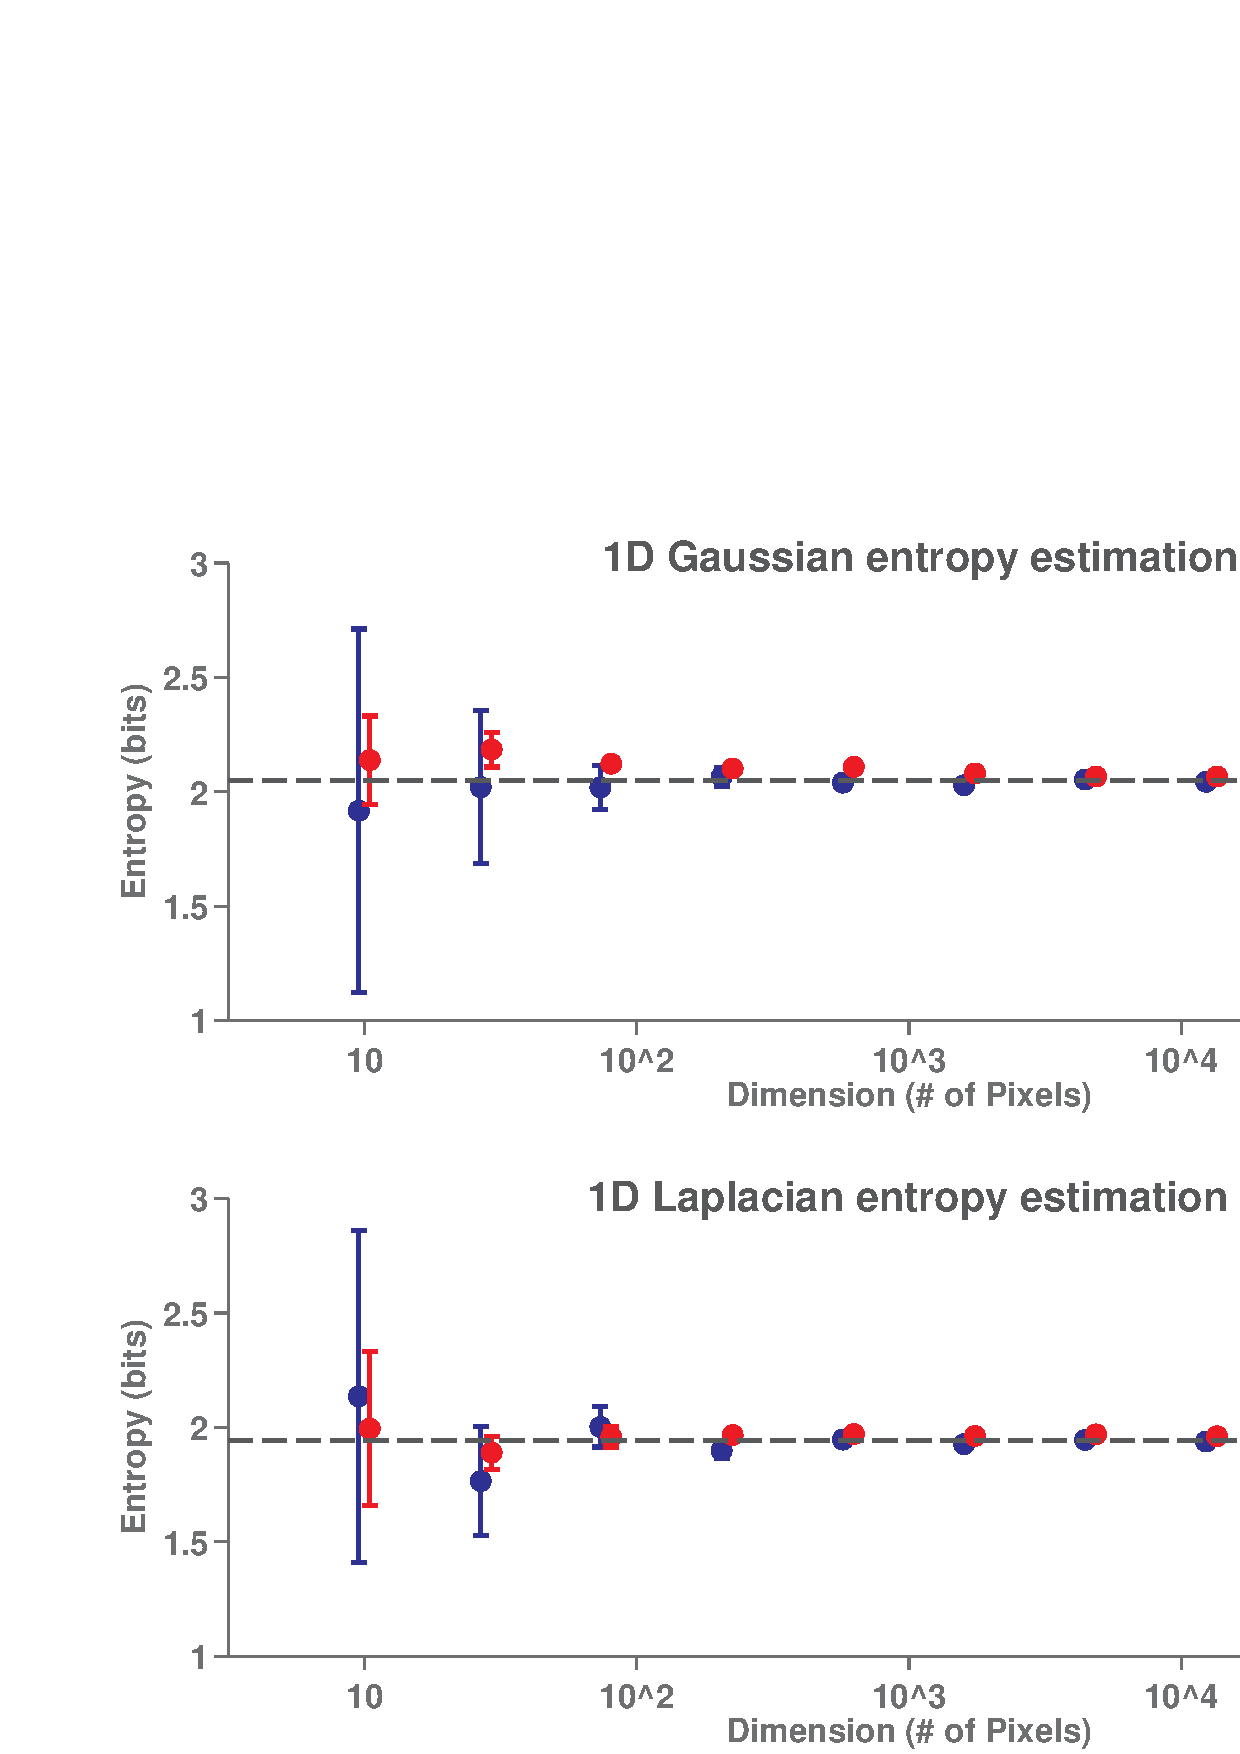
\includegraphics[width=0.95\linewidth]{1D.pdf}
   \caption{1D entropy estimation. Estimation using kernel density (red) and nearest neighbor (blue) methods, for samples drawn from a Gaussian (top) and Laplacian (bottom) as a function of the number of samples. Error bars are the variance in the estimate over 25 samples. The red/blue points are shown slightly offset for clarity.}
\label{fig:1D}
\end{center}
\end{figure*}

\begin{figure}[h]
\begin{center}
%\fbox{\rule{0pt}{2in} \rule{.9\linewidth}{0pt}}
   \includegraphics[width=1.0\linewidth]{ND.pdf}
   \caption{N-dimensional entropy estimation. The nearest neighbor method converges to the true entropy (for Gaussian distributions) quickly with increasing sample sizes.}
\label{fig:ND}
\end{center}
\end{figure}

\subsection{Maximum entropy}
With confidence in the nearest neighbor algorithm, I then turned to estimate entropy of image patches. First, I wanted to place a maximum bound on the entropy (in bits per pixel). From information theory, we know that the Gaussian distribution is the one with maximum entropy for a given mean and covariance. Here, I fit Gaussian models to image patches by estimating the covariance, and then computed the entropy of the Gaussian model analytically. Note that this is a pretty poor bound, as the distribution of image patches is highly sparse and not well fit by a Gaussian. However, it is still a useful exercise as it provides a ceiling for future estimates. I computed this "maximum entropy" for patch sizes ranging from $1\times 1$ to $7\times 7$ pixels, shown in Figure \ref{fig:gaussian}. I normalized by the dimension of the patch (the y-axis is bits per pixel) to compare across increasing dimensionality. Note that if the samples were truly normally distributed at each stage, we would expect a fixed entropy in bits per pixel. Here, we see that for natural distributions, we need to increase the dimensionality before this starts to converge. The maximum entropy estimated here for images is around \textbf{9 bits per pixel}.

\begin{figure}
\begin{center}
%\fbox{\rule{0pt}{2in} \rule{.9\linewidth}{0pt}}
   \includegraphics[width=1.0\linewidth]{maxent.jpg}
   \caption{Entropy of Gaussian models of image patches. A Gaussian model of image patches was fit using 5000 samples for different patch sizes, the entropy of the Gaussian is then computed analytically given the covariance matrix.}
\label{fig:gaussian}
\end{center}
\end{figure}

\subsection{Entropy of raw image patches}
The advantage of the nearest neighbor method is that it allows for estimation of the entropy of higher dimensional distributions.
I then applied the nearest neighbor estimation method directly to the ensemble of natural images. For increasing patch sizes (ranging from $1\times 1$, or single pixels, to $4\times 4$, a 16-dimensional distribution), I computed entropy as a function of the number of samples obtained, going up to a million samples. The results are summarized in the left plot of Figure \ref{fig:entropy}. Unlike the Gaussian high-dimensional example in Figure \ref{fig:ND}, the entropy estimates here did not converge for the larger patch sizes ($3\times 3$ and $4\times 4$). However, the estimate did converge for the 4-dimensional distribution of $2\times 2$ patches, to just over \textbf{6 bits per pixel}. This quantifies the reduction in entropy compared to single pixels, which have an entropy of almost \textbf{9 bits per pixel}. Note that these are much smaller than the maximum bound from Figure \ref{fig:gaussian}. To compute these estimates, I ran the algorithm on the Corn computing cluster. The runtimes for the computation are shown in the right plot of Figure \ref{fig:entropy}. Unfortunately, runtimes quickly grow as a function of sample size, and start to separate for the different dimensionality as well. In order to accurately measure the entropy of high dimensional distributions, we would need many samples and a faster way of computing pairwise Euclidean distances.

\begin{figure*}[h]
\begin{center}
%\fbox{\rule{0pt}{2in} \rule{.9\linewidth}{0pt}}
   \includegraphics[width=1.0\linewidth]{entropy.pdf}
   \caption{Entropy estimation of natural image patches. Estimates (left) converge for $1\times 1$ and $2\times 2$ pixel patches. Note the drop in entropy, indicative of considerable redundancy, for increasing patch sizes. Runtime (right) approaches more than 10 hours for sample sizes of $10^6$, and appears to be growing roughly linearly on the log-log plot.}
\label{fig:entropy}
\end{center}
\end{figure*}

\subsection{Projection onto basis vectors}
Given that we can only easily estimate the entropy for distributions of dimension 4 or fewer, I wanted to see what the entropy was for images projected onto a low-dimensional basis set. Using the ICA and PCA bases from Figure \ref{fig:bases}, I estimated the entropy of natural image patches projected onto this basis set. The results are summarized in Figure \ref{fig:projent}. The projection onto 42 learned basis functions are shown for ICA (blue) and PCA (red). The ICA bases are randomly assorted since they are learned together but the PCA bases are sorted according to the eigenvalue associated with the eigenvector. Interestingly, the projection onto ICA basis vectors has considerably more entropy than the projection onto the PCA basis set, which lets us quantify exactly how much more information can be captured with basis learned using the ICA objective function (finding independent components) compared to the PCA objective function (removing 2nd order correlations). This is also a quantification of the existence of higher-order statistical structure in natural images.

\begin{figure*}[h]
\begin{center}
%\fbox{\rule{0pt}{2in} \rule{.9\linewidth}{0pt}}
   \includegraphics[width=1.0\linewidth]{projent.pdf}
   \caption{Entropy estimation of image patches projected onto PCA and ICA basis vectors. Basis vectors were learned from $32\times 32$ pixel patches using principal and independent components analysis. New samples were then projected onto this basis set and the entropy of each projection was estimated separately. Projection onto PCA bases (red) are indexed by decreasing eigenvalue, ICA indices are arbitrary. An increase in the entropy is seen from the projection onto ICA bases compared with PCA bases.}
\label{fig:projent}
\end{center}
\end{figure*}

\subsection{Entropy of the joint distribution of projections onto oriented filters}
The fact that basis functions that are learned by ICA (as well as sparse coding, and other related algorithms) are oriented is one fascinating property of natural images.
Here, I test one metric of how important orientation is for feature description, using entropy estimation.
I projected $32\times 32$ pixel patches onto two Gabor receptive fields, of different orientations.
Then, I estimated the entropy of the resulting 2D distribution using the nearest neighbor algorithm, as a function of $\theta$, the angle between the receptive fields.
For a baseline comparison, I computed the same quantity for Gaussian noise projected onto the same basis set.
This gives us a way of quantifying the redundancy between joint filters in an ICA-like basis for natural images.
The results are summarized in Figure \ref{fig:jointent}.
I find that the change in orientation actually doesn't contain strong redundancies, as the shapes of the curves in Figure \ref{fig:jointent} are almost identitcal. Note that we expect the entropy to vary somewhat as a function of the difference in angle, as the filters themselves become more correlated - hence using white noise projected onto the bases as a baseline. Since we do not see a reduction in entropy for some angle difference, it seems as if two Gabor functions at the same point in space but with different orientations truly does provide an independent representation of image patches.

\begin{figure*}[h]
\begin{center}
%\fbox{\rule{0pt}{2in} \rule{.9\linewidth}{0pt}}
   \includegraphics[width=1.0\linewidth]{jointent.pdf}
   \caption{Entropy estimation of natural image patches. Estimates (left) converge for $1\times 1$ and $2\times 2$ pixel patches. Note the drop in entropy, indicative of considerable redundancy, for increasing patch sizes. Runtime (right) approaches more than 10 hours for sample sizes of $10^6$, and appears to be growing roughly linearly on the log-log plot.}
\label{fig:jointent}
\end{center}
\end{figure*}

\section{Conclusions and Future Work}
In this project, I have applied methods of entropy estimation (specifically, nearest neighbor techniques) to understanding the statistics of natural image patches. Besides being an interesting class of signals outright, understanding the statistical structure of natural images would help computer vision in giving us better priors statistical inference models as well as serving as a baseline for both compression schemes and comparing redundancy reduction algorithms. Here, I was able to estimate the entropy of natural image patches using the nearest neighbor technique. In addition, I compared the entropy of image patches projected onto basis functions learned from image ensembles, and found a strong increase in entropy of image patches projected onto ICA bases vs PCA bases.

Looking ahead, it would be interesting to take advantage of parallel GPU computing to comptue nearest neighbor distances. This would drastically reduce the run time and hopefully allow for entropy estimation of larger image patches. Due to long range correlations found in images, we should not expect to be able to estimate the true entropy of images using small patches. In addition, one could further characterize the entropy of images projected onto different bases, or look at joint distributions of projections onto different pairs of basis vectors. Here, I looked at the joint distribution onto Gabor bases with different orientations, but one might expect to find more redundancy between Gabors under translation or scaling.

In summary, understanding natural image statistics is important in our understanding of vision due to the non-trivial statistical structure found in image patches. One way of illuminating such structure is through entropy estimation, which allows us to quantify redundancy found in image patches. From a broader perspective, however, we will need many similar lines of attack to real deal with the high-dimensional statistical structure of images.

%\section{Future Work}
%Low-D projections, compute entropy


%\section{Criteria}
%• What is the computer vision problem that you will be investigating? Why is it interesting?

%• What image or video data will you use? If you are collecting new datasets, how do you plan to collect them?

%• What method or algorithm are you proposing? If there are existing implementations, will you use them and how? How do you plan to improve or modify such implementations?

%• Which reading will you examine to provide context and background?

%• How will you evaluate your results? Qualitatively, what kind of results do you expect (e.g. plots or figures)? Quantitatively, what kind of analysis will you use to evaluate and/or compare your results (e.g. what performance metrics or statistical tests)?

%\section{Introduction}

%Please follow the steps outlined below.
%\vspace{3cm}

%-------------------------------------------------------------------------
%\subsection{Language}

%All manuscripts must be in English.

%%-------------------------------------------------------------------------
%\subsection{The ruler}
%The \LaTeX\ style defines a printed ruler which should be present in the
%version submitted for review.  The ruler is provided in order that
%reviewers may comment on particular lines in the paper without
%circumlocution.  If you are preparing a document using a non-\LaTeX\
%document preparation system, please arrange for an equivalent ruler to
%appear on the final output pages.  The presence or absence of the ruler
%should not change the appearance of any other content on the page.  The
%camera ready copy should not contain a ruler.

%\subsection{Mathematics}

%Please number all of your sections and displayed equations.  It is
%important for readers to be able to refer to any particular equation.  Just
%because you didn't refer to it in the text doesn't mean some future reader
%might not need to refer to it.  It is cumbersome to have to use
%circumlocutions like ``the equation second from the top of page 3 column
%1''.  (Note that the ruler will not be present in the final copy, so is not
%an alternative to equation numbers).  All authors will benefit from reading
%Mermin's description of how to write mathematics.%: \url{http://www.cvpr.org/doc/mermin.pdf}.

%\subsection{Miscellaneous}

%\noindent
%Compare the following:\\
%\begin{tabular}{ll}
 %\verb'$conf_a$' &  $conf_a$ \\
 %\verb'$\mathit{conf}_a$' & $\mathit{conf}_a$
%\end{tabular}\\
%See The \TeX book, p165.

%The space after \eg, meaning ``for example'', should not be a
%sentence-ending space. So \eg is correct, {\em e.g.} is not.  The provided
%\verb'\eg' macro takes care of this.

%When citing a multi-author paper, you may save space by using ``et alia'',
%shortened to ``\etal'' (not ``{\em et.\ al.}'' as ``{\em et}'' is a complete word.)
%However, use it only when there are three or more authors.  Thus, the
%following is correct: ``
   %Frobnication has been trendy lately.
   %It was introduced by Alpher~\cite{Alpher02}, and subsequently developed by
   %Alpher and Fotheringham-Smythe~\cite{Alpher03}, and Alpher \etal~\cite{Alpher04}.''

%This is incorrect: ``... subsequently developed by Alpher \etal~\cite{Alpher03} ...''
%because reference~\cite{Alpher03} has just two authors.  If you use the
%\verb'\etal' macro provided, then you need not worry about double periods
%when used at the end of a sentence as in Alpher \etal.

%For this citation style, keep multiple citations in numerical (not
%chronological) order, so prefer \cite{Alpher03,Alpher02,Authors06} to
%\cite{Alpher02,Alpher03,Authors06}.

%\begin{figure*}
%\begin{center}
%%\fbox{\rule{0pt}{2in} \rule{.9\linewidth}{0pt}}
   %\includegraphics[width=0.8\textwidth]{gaussian_1D.png}
   %\caption{Entropy estimation of a normal distribution.}
%\end{center}
%\label{fig:g1d}
%\end{figure*}

%\begin{figure*}
%\begin{center}
%%\fbox{\rule{0pt}{2in} \rule{.9\linewidth}{0pt}}
   %\includegraphics[width=0.8\textwidth]{nongaussian_1D.png}
   %\caption{Entropy estimation of the distribution of pixel intensities in natural images.}
%\end{center}
%\label{fig:ng1d}
%\end{figure*}
%------------------------------------------------------------------------
%\begin{table}
%\begin{center}
%\begin{tabular}{|l|c|}
%\hline
%Method & Frobnability \\
%\hline\hline
%Theirs & Frumpy \\
%Yours & Frobbly \\
%Ours & Makes one's heart Frob\\
%\hline
%\end{tabular}
%\end{center}
%\caption{Results.   Ours is better.}
%\end{table}

%-------------------------------------------------------------------------
%\subsection{Illustrations, graphs, and photographs}

%All graphics should be centered.  Please ensure that any point you wish to
%make is resolvable in a printed copy of the paper.  Resize fonts in figures
%to match the font in the body text, and choose line widths which render
%effectively in print.  Many readers (and reviewers), even of an electronic
%copy, will choose to print your paper in order to read it.  You cannot
%insist that they do otherwise, and therefore must not assume that they can
%zoom in to see tiny details on a graphic.

%When placing figures in \LaTeX, it's almost always best to use
%\verb+\includegraphics+, and to specify the  figure width as a multiple of
%the line width as in the example below
%{\small
   %\usepackage[dvips]{graphicx}
   %\includegraphics[width=0.99\linewidth]{gaussian_1D.png}
%}


%-------------------------------------------------------------------------
%\subsection{Color}

%Color is valuable, and will be visible to readers of the electronic copy.
%However ensure that, when printed on a monochrome printer, no important
%information is lost by the conversion to grayscale.

{\small
\bibliographystyle{ieee}
\bibliography{egbib}
}

\section{Appendix}
I certify that this project is my own original work. This project is not part of larger work from another class or lab.
%If your course project is part of a larger project from another class or research lab, please fill in this section and clearly spell out the following items:

%\begin{enumerate}
%\item  Explicitly explain what the computer vision components are in this course project;
%\item  Explicitly list out all of your own contributions in this project in terms of:
	%\begin{enumerate}
	%\item ideas
	%\item formulations of algorithms
     %\item software and coding
	%\item designs of experiments
	%\item analysis of experiments
	%\end{enumerate}
%\item Verify and confirm that you (and your partner currently taking CS231A) are the sole author(s) of the writeup.
%Please provide papers, theses, or other documents related to this project so that we can compare with your own writeup.
%\item Please explicitly list out:
	%\begin{enumerate}
	%\item Is this project shared with some other course? If so, what class the project is being shared with (for all members of the team)
	%\item The exact contribution of each person
	%\item The exact portion of the project that is being counted for CS231A
	%\end{enumerate}
	%Failure to do the above is an honor code violation.
%\end{enumerate}
\end{document}
